% ------------------------------------------------------------------------------
% Chapter 3

% ------------------------------------------------------------------------------

\chapter{Markov Chain Model for Text} % enter the name of the chapter here
\label{cha:markov_chain_text} % enter the chapter label here (for cross-referencing)

We shall now delve deeper into how Markov Chains can be effectively used with texts, and more specifically, Novels written by famous authors. Instead of traditional Markov Chains, we shall be using a combination of Bayes' Formula as well as Markov Chain probability distributions with a character level distinction. What we saw in the previous section is how Markov Chains connect different nodes, through edges with a certain weightage for each edge going from any Node A to Node B.

A short summary of how we shall perform Markov Chain Analysis with Novels is by creating a probability distribution transition matrix of all unique characters in each novel, using those probabilities as our edge weightage in Markov Chains, then finally train, test, and predict which text was written by a particular author.

\section{Character Tokenization} % enter the name of the section here
\label{sec:tokenization} % enter the section label here (for cross-referencing)

\textbf{Tokenization is essentially splitting a phrase, sentence, paragraph, or an entire text document into smaller units, such as individual words or terms}. In true essence, when working with large datasets, we tokenize all the text into small parts, for a type of batch processing. Since our process is restricted to working with unique characters, we shall be breaking words into smaller parts. Given a character sequence and a defined document unit, tokenization is the task of chopping it up into pieces, called tokens , perhaps at the same time throwing away certain characters, such as punctuation. \textcite{manning:2008}.

In NLP, textual data has been traditionally segmented into “sentences” (or “utterances”, etc.) and
“words” due to linguistic motivations and technical constraints. The macroscopic units (“sentences”) are often considered independently from one another and themselves segmented into microscopic units. The definition of these microscopic units has always been a matter of approximation and compromise. On the one hand, these units receive linguistic annotations (e.g. part-of-speech tags, morphosyntactic annotation, syntactic dependency information), which would require them to be linguistically motivated units. On the other hand, a large range of phenomena makes it highly non-trivial to identify and even consistently define linguistic units, denoted by the Morphological Annotation Framework (MAF) ISO standard as word forms. \textcite{DBLP:journals/corr/abs-2112-10508}.

Delving deeper, the main goal of Tokenization is building a vocabulary of any given text. This vocabulary is not only limited to words. It could be characters, phrases, or even sentences. Taking an example of speeches by different world leaders, the same message can be relayed by various leaders in completely different languages, dialects, or even the same language using synonyms, and holding unique styles in their speeches. Each separate and unique piece of text, character, word, or phrase is generally known as a \textbf{Token}. In general, when dealing with medium to large sets of texts, only 3 types of tokens are broadly used, which are classified as follows:

\begin{enumerate}
    \item \textbf{Characters}
    \item \textbf{Subwords} \textit{(A good example of sub-words would be happy, which is the root for multiple words, such as happiness, happily, happiest, happier, and happinesses. Thus, all these words would be considered a part of the root word in a tree word-mapping structure).}
    \item \textbf{Words} \textit{(In word tokenization, we are not working with word stemming or lemmatization. These processes fall under the subword tokenization structure and helps identify a complete vocabulary instead of small words or characters).}
\end{enumerate}

In terms of a quick visualization, here is how all three tokenization processes are implemented.

\begin{figure}[H]
	\begin{center}
		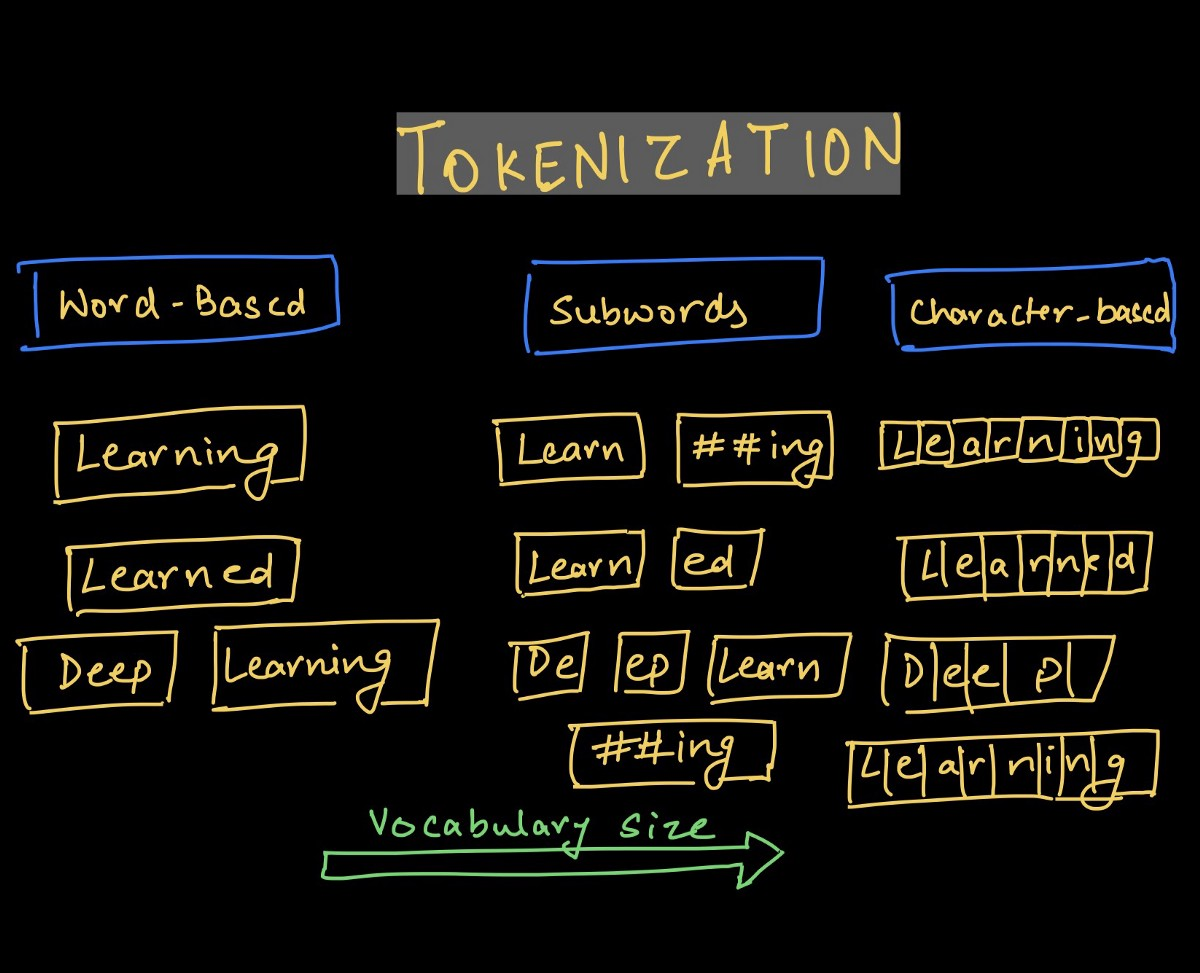
\includegraphics[width = 0.8\textwidth]{Images/tokenization.jpeg} % enter the filename here
		\caption{This is a quick example how character, subword and word tokenization works}
		\label{fig:tokenization-types}
	\end{center}
\end{figure}


If we deal with unique words or subwords, the number of tokens shall be much higher, leading to a much higher requirement of memory, space and computing power. In general working though, huge data models are trained on super-computers (as is the example of language translation of Google), then the model is released to the public, which constant upgrades and retraining taking place on the go.

Tokenization is the basic building block of any Natural Language Processing problem in machine learning. It is the most common process of solving any text prediction, one-hot embedding, or word-embedding problem, along with accessing raw text. 

One major problem also witnessed in Tokenization is the \textbf{OOV} (Out Of Vocabulary) issue. This causes the trained model to miss out on certain characters, words or subwords missed out during the training phase and are thus, encountered in the testing phase. This leads to the model not consisting of some tokens, causing errors in the prediction model. \textcite{tokenization_nlp_analyticsvidhya} .
However, these untrained tokens in words are generally solved by replacing the never-seen-before tokens with an \textit{$<$unknown token$>$} identifier. Since these words or characters are very rare in the main entire dataset, they are generally considered to have a very minuscule to nil effect on the final model. This would help in making sure the model is clean when tested, and does not create any out-of-memory error trying to retrain the same model upon revisitation.
 
\subsection{Character Tokenization} %enter the name of the subsection here
\label{sec:token_characters} % enter the subsection label here (for cross-referencing)

Characters are not limited to just English letters. It could be special characters like brackets({}, (), []), colons or semi-colons, numbers, etc. This breaks down the complete dataset into its most fundamental elements, creating a character-wise probability distribution that acts as the character weightage for our Markov Chain edges and nodes.

As discussed in previous sections and what shall be seen in the next sections we shall be utilizing character tokens are part of this project. The reason for this being we wish to delve deeper into how different novelists and authors use unique characters in their books. A detailed analysis of this shall be available in later sections as well. 

This trick in NLP can be considered quite useful when dealing with a smaller memory for the training model, and the size of the dataset would have a much lesser requirement of RAM or GPU for data processing. This is because characters, which can include letters from different languages, special characters such as semi-colons or commas, and numerical characters can be limited to maybe a maximum of a couple of hundred unique tokens.
Now, while this technique is much lower computationally expensive, character tokenization has a few drawbacks on its own.

\begin{itemize}
    \item Character tokens solve the OOV problem but the length of the input and output sentences increases rapidly as we are representing a sentence as a sequence of characters. As a result, it becomes challenging to learn the relationship between the characters to form meaningful words.
    \item If a single character is missed out from the training dataset, the actual relationship of the character with other tokens would be completely lost as the previously-not-seen character would be considered an \textit{$<$unknown token$>$}.
\end{itemize}

\subsection{Subword Tokenization}
\label{sec:token_subwords}

The core concept behind subwords is that frequently occurring words should be in the vocabulary, whereas rare words should be split into frequent subwords. Eg. The word “refactoring” can be split into “re”, “factor”, and “ing”. Subwords “re”, “factor” and “ing” occur more frequently than the word refactoring, and its overall meaning is also kept intact. \textcite{subwords_tokenization}. 

Since a majority of this project is focused on character tokenization and not subwords, we shall briefly understand all the different types of active subword tokenizations.

For reference to how subwords are broadly used, these are some of the most widely used techniques.

\begin{itemize}
    \item \textbf{Byte-Pair Encoding}, i.e., BPE was introduced in the article, \textcite{DBLP:journals/corr/SennrichHB15}, which explains how we can use Neural Machine Translations and extract all the words into an occurrence-based encoding, leading to either a word-wise or character-wise byte-pairing. Byte Pairing, however, has a distinction between train and test datasets, and would end up including some $<$unknown tokens$>$ in the test set.
    \item \textbf{WordPiece Tokenization}, works similar to Byte-Pair Encoding, with the exception that all the characters or words are already included in the vocabulary. This completely eradicates the need for unknown token generation and maximizes the likelihood of the training data and minimizes any training loss.
    \item \textbf{SentencePiece Tokenization}, does not treat space as a separator, instead, it takes the string as input in its original raw format, i.e. along with all spaces. It then uses BPE or unigram as its tokenizers to construct the vocabulary. In this case, words are pre-tokenized with a special character, which could be \textunderscore , or -, or any other distinctive character token.
\end{itemize}

\subsection{Word Tokenization}
\label{sec:token_words}

Word Tokenization, is among the most widely used algorithm in NLP, as it stores the essense of words in sentences while a model is trained. During word tokenization, there is no change in the final words, rather, stop words are removed, word-stemming and lemmatization takes place and root-words are separated from the actual text. A number of techniques, such as GloVe, Word2Vec, are used for the vectorization of words into word embeddings for a graphical representation, based on the overall probability of occurance in pre-trained or newly trained NLP models.

When dealing with words, there are a number of issues one can face. Some of them are as follows:

\begin{itemize}
    \item \textbf{OOV Words}, also stated above as \textbf{Out-Of-Vocabulary} words, certain words tend to be rare in the dataset. In order to handle these missing words, only the Top-K Frequent words are included in the dictionary and the remaining missing words are handled as \textit{$<$unknown token$>$}.
    \item \textbf{$<$unknown token$>$}, are missing words, which have been replaced in the vocabulary, and are very rare. However, the word mapping is lost in case of UNK tokens.
    \item \textbf{Large Vocabulary}. In this issue, most of the models we see today have been trained over huge corpus of text, which could range from twitter to novels to article datasets. In order to improve any of the models, a large amount of memory would be needed to train these models all over again.
\end{itemize}

Due to these drawbacks, we also sometimes focus on character tokenization of small datasets, which would preserve the overall structure of words, but ends up missing out on sentence formation and containing the meaning of words.


% ------------------------------------------------------------------------------
% Referencing examples
% ------------------------------------------------------------------------------
\section{Custom Bayes' Rule Implementation}
\label{sec:custom-bayes-implementation}

From what we learnt in the previous chapter, Naive Bayes' formula is very useful calculating underlying probabilities of 'A' given 'B'. 

Since we are using character tokens for our novels, we work with a custom Bayes' formula. Before we go on to the custom formula, let us consider an example.

\begin{equ}[!ht]
  \begin{equation}
    \label{eq:bayes-2}
    P(\theta|\textbf{D}) = \frac{P(\theta ) * P(\textbf{D} |\theta)}{P(\textbf{D})} ~~~~~|| I,
  \end{equation}
\caption{where {\texttheta} is the target and \textbf{D} is the feature}
\end{equ}

While in a normal Naive Bayes' theorem we have one target and one feature, we work with a custom form while working over our character tokenization problem, creating a probability matrix for each novel we work with. However, with a customized Bayes' Theorem, we work with multiple features. Let us consider an example for the same.

\begin{equ}[!ht]
  \begin{equation}
    \label{eq:characters_all}
    x_{1}, x_{2}, ..., x_{n} \in \textbf{A}
  \end{equation}
\caption{where $x_{k}$ are all the distinct characters and \textbf{A} are all real characters.}
\end{equ}

In general, when dealing with a specific language, the vocabulary is restricted to the characters found within that language. For example, with English, we are dealing with a vocabulary of about 94 characters, which includes special characters, numerals, capital and small letters. An extended example is provided in the image \ref{fig:english-characters}. With it, we can understand how each character would have a different weightage, once we have a broader understanding of the complete vocabulary for our custom Bayes' Rule.

\begin{figure}[H]
	\begin{center}
		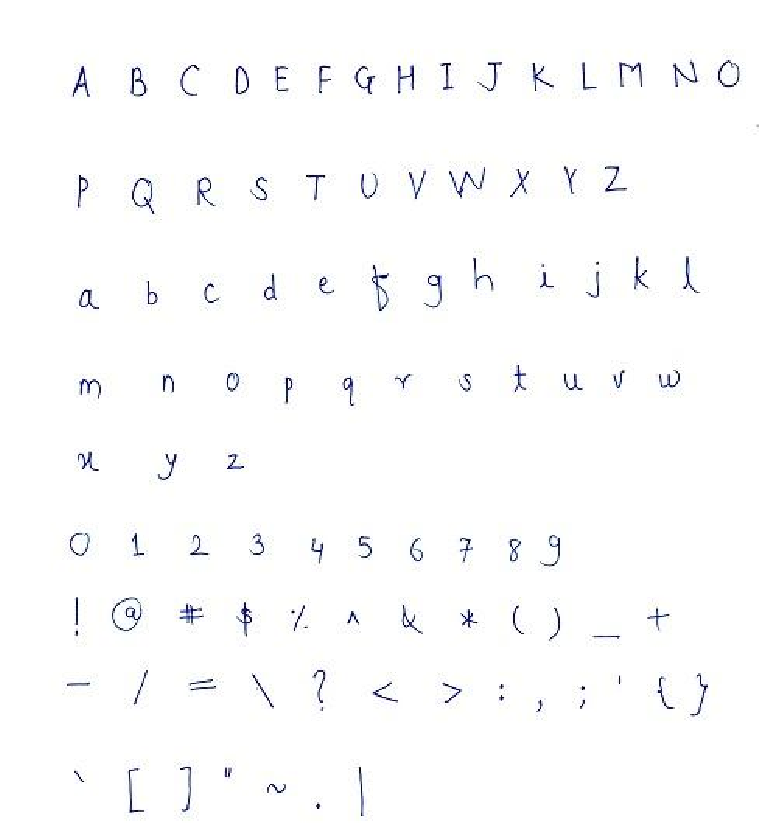
\includegraphics[width = 0.7\textwidth]{Images/english_characters.png} % enter the filename here
		\caption{An exhaustive list of all English characters \cite{english_characters}.}
		\label{fig:english-characters}
	\end{center}
\end{figure}

Keeping in mind the true formula of Bayes' Rule from the equation \ref{eq:bayes-2}, our target \texttheta is the variable for our novel we are trying to predict, and \textbf{D} is/are the features we have, i.e, our character sets. For each target, the overall characters shall remain the same as the number of characters does not budge. Thus, our features remain static and the prediction algorithm works over the probabilities. 

Bayes' Formula, which works over probabilities on the occurrences, determines the extent to which an event is supposed to occur. However, the summation of all the probabilities of an event always sums up to 1.


\begin{equ}[!ht]
    \begin{equation}
        \label{eq:probabilities_sum}
        \sum_{a \in \textbf{A}} P_x^{\left ( i \right )} = 1
    \end{equation}
\caption{$\forall$ events 'i' and features 'x'}
\end{equ}

Now with this equation, we move ahead with an assumption that all probabilities sum up to 1 for each event in the matrix. After this, we shall be able to move ahead with the overall structure of our Custom Naive Bayes' theorem, which can be a good predictor of the occurrence of randomized conditions. With this assumption, let us consider our custom Bayes' formula.

\newline

\begin{equ}[!ht]
    \begin{equation}
        \label{eq:custom_bayes_p1}
        P \left ( i | x_{1}, x_{2}, \cdots, x_{n} \right ) &= \frac{P \left (x_{1}, x_{2}, \cdots, x_{n} | i \right ) . \pi \left ( i \right )}{P \left (x_{1}, x_{2}, \cdots, x_{n} \right )}
    \end{equation}
\caption{$\forall$ events 'i' and features 'x', a custom Bayes' Theorem}.
\end{equ}

In the equation \ref{eq:custom_bayes_p1}, we mainly deal with probabilities. 
\begin{itemize}
    \item $\pi \left ( i \right )$ is the probability of an event 'i' occurring.
    \item $P \left ( i | x_{1}, x_{2}, \cdots, x_{n} \right )$ is the probability of event 'i' occurring given $x_{1}, x_{2}, \cdots, x_{n}$ occur.
    \item $P \left (x_{1}, x_{2}, \cdots, x_{n} | i \right )$ is the probability of $x_{1}, x_{2}, \cdots, x_{n}$ occurring given that event 'i' has already transpired.
\end{itemize}


Now, the denominator $P \left (x_{1}, x_{2}, \cdots, x_{n} \right )$, is just the probabilities of our features 'x' occurring over a given event. This means, however small the product of the probabilities be, they shall remain constant for the event 'i'. Similarly, $\pi_{i}$ is the probability of an event 'i' occurring and for all events, the probability shall remain constant. 

Thus, moving ahead, we can replace the equality with a proportionality instead since we have two variables that remain constant for an event 'i'. Thus, our new custom Bayes's Rule can be summarised as follows.

\begin{equ}[!ht]
    \begin{equation}
        \label{eq:custom_bayes_p2}
        P \left ( i | x_{1}, x_{2}, \cdots, x_{n} \right ) &\propto \Pi_{j = 1}^n P_{x_j}^{\left ( i \right )} . \pi \left ( i \right )
    \end{equation}
\caption{\textit{The R.H.S. is a product of all of the feature probabilities}}.
\end{equ}

Considering we would have to deal with values of the feature probabilities all ranging from [0, 1], the best option would be to take a log of the probabilities of $x_1, x_2, \cdots, x_n$ combined, and according to the product rule of log, we would just need to sum up the log probabilities individually. In terms of an equation, we state it at follows.

\begin{equ}[H]
    \begin{equation}
    \begin{split}
        \label{eq:custom_bayes_p3}
        \log_e \left ( P \left (x_{1}, x_{2}, \cdots, x_{n} | i \right ) \right ) &= \log_e \left ( \Pi_{j = 1}^n P_{x_j}^{\left ( i \right )} . \pi \left ( i \right ) \right ) \\
        &= \sum_{j = 1}^n \log_e P_{x_j}^{\left ( i \right )} + \text{Const.} \\
        &= \sum_{j = 1}^n \log_e P_{x_j}^{\left ( i \right )} - \max_{j} \log_e P_{x_j}^{\left ( k \right )}
    \end{split}
    \end{equation}
\caption{\textit{Log of a product leads to the summation over individual Logs}}
\end{equ}

A short summary of equation \ref{eq:custom_bayes_p3}, we obtain a $\textbf{Const.}$ upon taking the logarithm over $\pi \left ( i \right )$, we take the $\max_{j} \log_e P_{x_j}^{\left ( k \right )}$ as the constant because \textbf{each iteration would add an additional maximum value of and each event would have a new adjustment factor}. \textit{Please note, the maximum we take is over all the novels we are working alongside and not just a single character maximum}.

Now each of our Bayes' rule probabilities are stored as effective weights for our Markov Chain model's edges and useful for connecting nodes. We add the constant at the end of equation \ref{eq:custom_bayes_p3} so as to adjust for any bias. One key change we have made is adding a $\log_e$ to the custom rule. Thus, in order for this logic to function, we would need to take an exponent to revert back to the actual probability.

Finally, we can concise all the equations above in the next final equation, which becomes the basis of our complete project, \textbf{which is to predict which piece of text was authored by which novelist}. 

\begin{equ}[H]
    \begin{equation}
    \begin{split}
        \label{eq:final_custom_bayes}
        \log_e \left ( P \left (L | X_{1} = W, X_{2} = E \right ) \right ) &= \log_e \left ( P \left (X_{1} = W, X_{2} = E | L \right ) . P \left ( L \right ) \right ) \\
        &= \log_e ( P \left (X_{1} = W, X_{2} = E | L \right ) + \left(n . \log_e P \left ( L \right ) \right ) \pm  \log_e \left( Const. \right)
    \end{split}
    \end{equation}
\caption{\textit{Summarization of the custom formula for Bayes' Rule and Markov Chains}}
\end{equ}

There are multiple reasons why a log was the best solution. We shall state them as follows:

\begin{enumerate}
    \item Probabilities are always between [0, 1) and upon multiplying small numbers, ex: 0.01 * 0.001 = 0.00001, which would yield computationally insignificant results.
    \item With Logarithms at this step, we eliminate the possibility of a variable's impact in the final model going zero. Instead, that log converts the probability into a negative number for further calculations.
    \item Each event would have its own probability, and with negative logs, prediction over the test set shall be much easier.
\end{enumerate}

\section{Custom Bayes' Rule Example}
\label{sec:custom-bayes-example}

In this section, we shall see a quick example of how we would train a text dataset based on its probabilities and use Bayes' Rule to solve that issue. As we have seen in \ref{sec:custom-bayes-implementation}, each and every value needs to be given equal importance. Thus, we take a log of the values as lower values would end up being considered negligible by a simple model, and thus, result in data loss.

Let us show this as an example. 

Say we have two pieces of text and let's call them events. 
$ABCB$ and $BACCA$. Now, since we already know the length of the strings, and all the unique characters are present, we can easily compute their respective character probabilities. Let $ABCB$ be event 1 and $BACCA$ be event 2 for the purposes of our example.

\begin{equ}[H]
    \begin{equation}
    \begin{split}
        \label{eq:custom_train_example}
        Event_1 \\
        P\left(A\right)^{\left(1\right)} = 1/4 \\
        P\left(B\right)^{\left(1\right)} = 1/2 \\
        P\left(C\right)^{\left(1\right)} = 1/4 \\
        --------\\
        Event_2 \\
        P\left(A\right)^{\left(2\right)} = 2/5 \\
        P\left(B\right)^{\left(2\right)} = 1/5 \\
        P\left(C\right)^{\left(2\right)} = 2/5 \\
    \end{split}
    \end{equation}
\caption{\textit{Example of the Bayes' Rule above}}
\end{equ}

Consider the training examples we have. \textbf{ABCB} and \textbf{BACCA}, which we shall use in order to present generate an extremely elementary Markov Chain model. With this, we separate each text into its elemental units, i.e., characters. And then we calculate the probabilities of each character within each piece of text. Thus, ensuring the total probabilities sum up to 1. Now, we shall test a simple piece of text and then use it to possibly predict which sequence of characters works best with it.

Thus, we can next, calculate the probabilities from the information we calculated in equation \ref{eq:custom_train_example}. Let us consider we have a new piece of text, $BBC$, for which we need to predict which event did this test tentatively originate from.


\begin{equ}[H]
    \begin{equation}
    \begin{split}
        \label{eq:custom_test_example}
        Test \\
        P\left(BBC | event_1\right) = 1/2 * 1/2 * 1/4 = 1/16 = 0.0625 \\
        P\left(BBC | event_1\right) = 1/5 * 1/5 * 2/5 = 2/125 = 0.016 \\
        --------\\
        Now, 0.0625 > 0.016
    \end{split}
    \end{equation}
\caption{\textit{Example of the Bayes' Rule above}}
\end{equ}

From both these examples above, we can quickly see that $P \left ( 'BBC' | event_{1} \right )$ gives an yield of 0.0625 probability whereas the $P \left ( 'BBC' | event_{2} \right )$ shows us this probability of occurrence goes down to 0.016. Thus, we can consider that 'BBC' could be predicted as being a part of event 1 rather than event 2 in our machine learning model.

Since our target was to use character-level Markov Chains, and the key characteristic of any Markov Chain model is that each weight going out of a node sums up to one, we perform this over a complete novel, in order to better capture the results of how prediction could work for a particular piece of text when dealing with a number of different authors. In order to predict the final outcome in predicting the right novel, we shall create a transition matrix, which is depicted as a probability matrix for each novel corresponding to each character. 

\section{Laplacian Smoothing}
\label{sec:laplace-smoothing}

In general, Laplace Smoothing is also termed as Additive Smoothing. In a broader understanding of the term, Laplace Smoothing is used in order to \textbf{smooth categorical data}. Let us consider this with the help of an equation.
Let us consider we have a list of observations, $X = < x_1, x_2, \cdots, x_p>$ with p-dimensions, and n possible scenarios or possible state spaces. Thus, we just add an additional value $\alpha$ to all the values, in order to avoid any zero values occurring in the text. In terms of the equation, it can be explained below:

\begin{equ}[H]
    \begin{equation}
    \begin{split}
        \label{eq:laplacian-smoothing-generic}
        \hat{\theta}_i = \frac{x_i + \alpha}{n + \left(\alpha * d\right)}
    \end{split}
    \end{equation}
\caption{\textit{$\forall i = \left(1, 2, \cdots, d\right)$}}
\end{equ}

where $\hat{\theta}_i$ is the estimator and the smoothed count $\hat{x}_i = n\hat{\theta}_i$ and the \textit{pseudo-count} $\alpha > 0$ is a smoothing parameter. $\alpha = 0$ corresponds to no smoothing.
Additive smoothing is a type of shrinkage estimator, as the resulting estimate will be between the empirical probability (relative frequency) $\frac{x_i}{n}$, and the uniform probability $\frac{1}{d}$. In general, the value of our smoothing parameter $\alpha$ has to be 1 when dealing with categorical variables. But it could also be argued the value can be deemed lower and maintained much lower in order to ensure minimal to no impact on the probability distribution and the transition matrices which need to be designed for the model.

Additionally, we shall see further in the working of our model that we use 1 as the Laplacian Smoothing constant in order to avoid the zero probabilities within the training set, such as to avoid any unseen occurrence of a value in the testing set, ensuring data loss is minimal.

Finally, Laplacian smoothing can be a very useful tool, when we are working with different sets of training, and testing data. Thus, when working with categorical data, we can work with the maximum value we are allowed to use. With 1, the value in and of itself would have a very minimal to absolutely no impact on the actual model but would ensure features are being accounted for, no data loss takes place during training. 


\section{Custom Testing over Prediction}
\label{sec:custom-testing}

Now, theoretically, we shall be going over how we would calculate our results, specifically the scores a piece of text could achieve which would be close to the actual novel the text was picked up from. However, to explain it, let us consider we have a \textbf{Transition Matrix} \ref{eq:discrete-time-transition-matrix} ready for a piece of text, and in the case of our dissertation, let the piece of text belong to a particular author.

Let the text in question be denoted as $x_1, x_2, \cdots, x_n \in \{ A, B, C \cdots \}$, where all $x_1, x_2, \cdots, x_n$ would be a part of a random sequence $AVASD BGHGF MKIODF LPSD! \cdots$. Now, we can quickly define the transition matrix as follows, for a given author k.

\begin{equ}[!ht]
    \begin{equation}
    \begin{split}
        \label{eq:custom-transition-matrix}
        P^{k} = \left(
        \begin{array}{cccc}
        p_{AA}^{k} & p_{AB}^{k} & p_{AC}^{k} & \cdots \\
        p_{BA}^{k} & p_{BB}^{k} & p_{BC}^{k} & \cdots \\
        p_{CA}^{k} & p_{CB}^{k} & p_{CC}^{k} & \cdots \\
        \vdots & \vdots & \vdots & \ddots
        \end{array}
        \right)
    \end{split}
    \end{equation}
\caption{An example of the actual transition matrix we shall define}.
\end{equ}

Now, these are all probabilities of each element occurring in the training set. Thus, from our custom Bayes' Rule equation \ref{eq:custom_bayes_p3}, we can simply calculate the final probabilities with this given equation. And on the basis of our calculated log from equation \ref{eq:custom_bayes_p3}, we can predict the closeness of the data from the training set, along with that of the test set.


\begin{equ}[H]
    \begin{center}
    \begin{equation}
    \begin{split}
    \raggedright
        \label{eq:custom-test-results}
        log\left( P \left( X = \say{AVASD\space \cdots} | k \right) \right) &= \\
        log \left( p_{A}^{\left(k\right)} p_{AV}^{\left(k\right)} p_{VA}^{\left(k\right)} p_{AS}^{\left(k\right)} p_{SD}^{\left(k\right)} p_{D\cdots}^{\left(k\right)} \right) &= \\
        log\left(p_{A}^{\left(k\right)}\right) + log\left(p_{AV}^{\left(k\right)}\right) + log\left(p_{VA}^{\left(k\right)}\right) + log\left(p_{AS}^{\left(k\right)}\right) + log\left(p_{SD}^{\left(k\right)}\right) + log\left(p_{D<space>}^{\left(k\right)}\right) + \cdots
    \end{split}
    \end{equation}
    \end{center}
\caption{A final equation where we shall calculate our testing results}.
\end{equ}

Keep in mind that we shall be using dual and singular probabilities for a given piece of text. For the purposes of our model, we shall have the probabilities ready and then calculate individual log probabilities, sum them up over the test set and find which is the closest value for all of the books.

And once again, while we compare our results with equation \ref{eq:custom_bayes_p3}, and reduce the maximum out of all values for regularization, the maximum of $P\left( <text> | k\right)$ for all novels k would be considered as the regularization term.
